\subsection{Efficient General Lattice Generation and Rescoring \cite{Ljolje1999}}

This paper describes a lattice generation method that produces high-quality lattices with less than 10\% increased computation over standard \emph{Viterbi} decoding. The proposed method is closely related to previous lattice generation methods, but applies to more general network topologies.

\begin{figure}[h]
  \centering
  % Requires \usepackage{graphicx}
  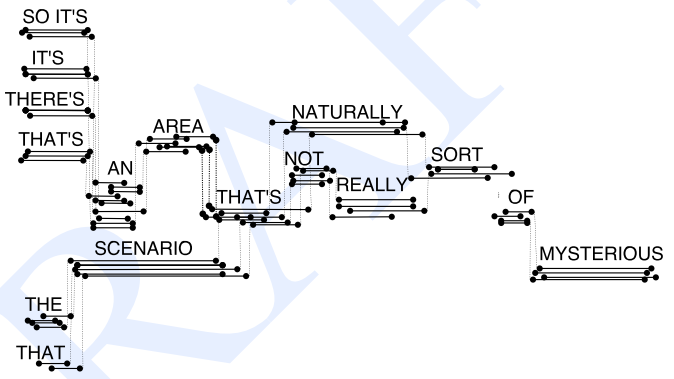
\includegraphics[width=.7\linewidth]{11_21_lattice.png}\\
  \caption{Example of a lattice}\label{fig:lattice}
\end{figure}

In this paper, a \emph{lattice} is defined to be a labeled, weighted, directed acyclic graph in which each complete path represents an alternative transcription hypothesis, weighted by its recognition score for a given utterance. However, it should be noted that there is no generally accepted single definition of lattice. Figure \ref{fig:lattice} shows an example of lattice (figure from Chapter 10 of Speech and Language Processing \cite{Jurafsky2006}).

In this paper, \emph{ASR networks} are represented as \emph{finite-state transducers}. These are labeled, weighted, directed graphs in which each arc $a$ has a source state $S(a)$, destination state $D(a)$, an input label $I(a)$, output label $O(a)$, and a weight $P(a)$. Here each input label is a context-dependent phone symbol, and each output label is a word. A complete path through such a transducer gives a legal sequence of words in the language model.

The recognition task can be characterized as finding a path $a = a_1,...,a_n$ that maximizes the joint probability of the acoustic and language models when applied to a given utterance:
$$\max_a P(\vec{x}[0, \tau], a) = \max_{a, t_1, ..., t_{n-1}}\prod_{i=1}^n P(\vec{x}[t_{i-1}, t_i] | I(a_i)) P(a_i).$$

The first factor represents the acoustic model likelihood for the context-dependent phone $I(a_i)$, and the second factor represents the language probability for that arc in the transducer $T$. Let $B(s)$ be the set of all paths in $T$ from the initial state to state $s$. Define
$$\alpha(s,t) = \max_{a \in B(s), t_1, ..., t_{k-1}} \prod_{i=1}^k P(\vec{x}[t_{i-1}, t_i] | a_i) P(a_i).$$
Then:
$$\max_{a} P(\vec{x}[0,t], a) = \max_{D(a)=s} p(a) [\max_{t' < t} P(\vec{x}[t',t]|I(a)) \alpha(S(a), t')].$$
In this way, the familia Viterbi recursion is factored into two nested loops: the outer loop considers each possible active arc $a$ ending in $s$, and the inner loop picks out the optimal start time $t'$.

The lattice generation algorithm consists of three main steps: 1) creates a context-dependent phone-to-word transducer lattice; 2) converts it to a word lattice; 3) prunes the lattice relative to the best scoring path.

In the first step, each state in lattice $L$ corresponds to a pair $(t,s)$ of a time frame in the recognition and a state from the transducer $T$. If during the Viterbi recursion, it has identified the optimal start time $t'$ for are $a$ ending in state $D(a)$ at time $t$, then a corresponding arc is added to $L$ from $(t', S(a))$ to $(t, D(a))$.

To convert the phone-to-word lattices to word lattices, it relies on the efficient implementations of the general finite-state operations. It deletes the input labels by the projection operator, and removes the $\epsilon$ arcs.

The final step is to prune the lattice relative to the best scoring path. The method is simple: the best score $\alpha(s)$ among paths from the initial state to state $s$ is found, as well as the best score $\beta(s)$ among paths from state $s$ to a final state. State for which $\alpha(s) + \beta(s) < \kappa \times \beta(s_0)$ are then pruned.

In the experimental section, it is shown that lattice generation requires typically less than 10\% additional computation time above one-best decoding. With the second pass, the proposed method is able to achieve a 3x real-time word error rate of 11.2\% on the Eval'95 test set. 